\vspace{-2in}
\chapter{Work Done}

\section{Theory}
In Cloud Computing, an organization has to decide whether it has to Self-execute or pay Rent for the computing facilities. Considering factors like execution time, the number of resources required, number of jobs in a batch and the waiting probability, forecasting is done to determine the strategy. Since these data are generally random in a Cloud environment, using forecasting methods that depend on seasonal data cannot be considered. Methods that rely on level and trend based data have been used \cite{TimeSeries}. Further, considering only current data, a game theoretic approach is applied which decides the optimal strategy for any situation.
\subsection{Utility Function}
A utility function translates outcomes into numbers such that the expected value can be used to calculate certainty equivalents for alternatives in a manner that is consistent with a decision maker's attitude toward risk taking \cite{Book}.\\
\begin{displaymath}
Utility = { \frac{e}{t_{avg}} + n^{1-p} \over s}
\end{displaymath}
where:\\
$e$ - Execution time of current job.\\
$t_{avg}$ - Moving average of the execution times of all the previous jobs in the batch.\\
$n$ - Number of resources required by the current job.\\
$p$ - Waiting probability.\\
$s$ - Batch size.\\
The strategy adopted is to maximize the utility. Taking into consideration resource utilization, execution time and throughput, all the factors of load balancing have been given weightage.
\begin{enumerate}
\item[(a)] $e \over t_{avg}$ deals with execution time and average previous throughput. 
\item[(b)] $n^{1-p}$ deals with resource allocation. If number of resources required is less then waiting probability tends to be less. The job gets executed faster because of lesser waiting probability. So to maximize utility; if $e \over t_{avg}$ is less, then this factor need to be higher to increase the utility value. Hence $n$ has been raised by a factor of $(1-p)$.
\end{enumerate}
The above terms are added because of this compensation, i.e., if one factor is less then the other factor is higher and vice-versa, and also because it is a consideration of all the factors of load balancing,  this operation gives each of these factors a non-trivial weightage in the utility function. Division by the batch size helps in maintaining uniformity between batches.
\subsection{Forecasting Methods}
Forecasting involves making projections about future performance on the basis of historical and current data. The need for forecasting stems from the time lag between awareness of an impending event or need and the occurrence of that event. Forecasting methods are applied to predict the future and depending on the data we can classify it into level-based, trend-based and seasonality-based.
\subsubsection{Exponential Smoothing}
Exponential smoothing forecasts are forecasts for an integrated moving average process; however, the weighting parameter is specified by the user rather than estimated from the data. Experience has shown that good values for the weighing parameter = $\alpha$ are between 0.05 and 0.3 \cite{SAS}.\\The single exponential smoothing operation is expressed by the formula :
\begin{displaymath}
FORECAST(t+1) = \alpha \ast demand(t) + (1-\alpha) \ast FORECAST(t)		 	 
\end{displaymath}
where:\\ 
$demand(t)$ - Current actual value of the series.\\
$FORECAST(t)$ - Forecast value at the current period.\\
$FORECAST(t+1)$ - Forecast of $demand(t+1)$.

\subsubsection{Holt's Method}
Holt's Method is a double exponential smoothing method used for forecasting, when there is a linear trend present in the data. The method requires separate smoothing constants for slope and intercept.
\begin{displaymath}
FORECAST(t+1) = a(t) + b(t)
\end{displaymath}
\begin{displaymath}
a(t) = \alpha \ast demand(t) +(1-\alpha) \ast (a(t-1) + b(t-1))
\end{displaymath}
\begin{displaymath}
b(t) = \beta \ast (a(t) - a(t-1) ) + (1-\beta) \ast b(t-1)
\end{displaymath}
where:\\
$a(t)$ - Level which represent the smoothed value up to and including the last data.\\
$b(t)$ - Slope of the line representing the trend.\\
$demand(t)$ - Current actual value of the series.\\
$FORECAST(t+1)$ - Forecast of $demand(t+1)$.\\
\subsection{Forecast Design}
For each batch, a forecasting method is applied with the existing utility values to compute the utility value for the next batch. The forecasting methods can depend on the trend present in these input utility data. If no trend is present, exponential smoothing can be applied and the presence of trend will shift the forecasting to Holt's Method.\\[0.2cm]
$\hspace*{3mm}/^\ast Choosing\hspace*{1mm}Forecasting\hspace*{1mm}Method^\ast/$\\
\begin{algorithmic}
\IF {$trend == true$}
	\STATE $method \gets Holt's\hspace*{1mm}Method$
\ELSE
	\STATE $method \gets Exponential\hspace*{1mm}Smoothing$ 
\ENDIF
\end{algorithmic}
\vspace{0.2cm}
The computed forecasted value is compared with the actual utility value of the batch (an average of the utility values of all the jobs in the batch) to understand the computing facilities required to execute the batch.\\[0.3cm]
$\hspace*{3mm}/^\ast Choosing\hspace*{1mm}Batch\hspace*{1mm}Strategy\hspace*{1mm}by\hspace*{1mm}Forecasting^\ast/$\\ 
\begin{algorithmic}
\IF {$forecast\hspace*{1mm}value < average\hspace*{1mm}utility$}
	\STATE $strategy \gets Rent$
\ELSE
	\STATE $strategy \gets Self-execute$
\ENDIF
\end{algorithmic}
\vspace{0.2cm}
When the value of forecast is obtained, the system prepares itself to provide computing facilities atmost equal to that of the utility value forecasted. So if the forecasted value is less than the actual utility value, then the system was not prepared to handle that load as it forecasted only lesser facilities . So the cloud owner pays rent to an external cloud who can provide the necessary computing facilities for executing the batch. If found otherwise, the cloud owner will execute the batch with the facility he owns.\\[0.2cm]
%game theory
\subsection{Game Theoretic Design}
Game theory is the formal study of conflict and cooperation. Game theoretic concepts apply whenever the actions of several agents are interdependent. The concepts of game theory provide a language to formulate, structure, analyze, and understand strategic scenarios.\\[0.2cm]
In this approach, two utility values are calculated for two waiting probabilities, $p_1$ and $p_2$ where $0<=p_1<=0.5$ and $0.5<p_2<=1$.The strategies of Rent and Self-execute then randomly take the $u_1$ and $u_2$ values:\\[0.3cm]
$\hspace*{3mm}/^\ast On\hspace*{1mm}Random\hspace*{1mm}Coin-toss^\ast/$\\
\begin{algorithmic}
\IF {$Coin-toss == 1$}
	\STATE $Rent \gets u_1$
	\STATE $Self-execute \gets u_2$
\ELSE
	\STATE $Self-execute \gets u_1$
	\STATE $Rent \gets u_2$
\ENDIF
\end{algorithmic}
\vspace{0.2cm}
The above random strategy can be interchanged without much effect. So, for each batch of jobs a matrix $M_{Batch Size\hspace*{0.5mm}X\hspace*{0.5mm}2}$ is created with utility values for Rent and Self-execute strategies. The maximum utility values for each strategy is then selected alongwith its corresponding rows resulting in a matrix $M'_{2\hspace*{0.5mm}X\hspace*{0.5mm} 2}$. A method of mixed strategy calculation is applied to $M'$ which chooses the strategy with the higher probability $p$.\\[0.2cm]

%standard deviation
\subsection{ Standard Deviation }
Standard deviation (represented by the symbol sigma, $\sigma$) shows how much variation or "dispersion" exists from the expected value. Standard deviation is commonly used to measure confidence in statistical conclusions.\\
\begin{displaymath}
\sigma = \sqrt{ \frac{1}{N} \sum_{i=1}^{N} (x_i-\mu)^2}
\end{displaymath}
The strategy given by forecasting and game theory may be different. In such a case, further decision has to be taken as to which strategy should be adopted. The method of standard deviation in each conflicting batch is applied about the points:\\[0.3cm]
$\mu_1\hspace*{0.5mm}=\hspace*{0.5mm}forecasted\hspace*{1mm}value$\hspace*{3.5mm}$/^\ast Forecast\hspace*{1mm} approach^\ast/$\\
$\mu_2\hspace*{0.5mm}=\hspace*{0.5mm}equilibrium\hspace*{1mm}value$\hspace*{2mm}$/^\ast Game\hspace*{1mm}Theory\hspace*{1mm}approach^\ast/$\\[0.3cm]
where equilibrium value is obtained as:
\begin{displaymath}
p\ast utility_p + (1-p) \ast utility_{1-p}
\end{displaymath}
The final strategy is given by the approach that has minimum standard deviation.\\[0.3cm]
$\hspace*{3mm}/^\ast In\hspace*{1mm}case\hspace*{1mm}of\hspace*{1mm}Conflict\hspace*{1mm}of\hspace*{1mm}Strategies^\ast/$
\begin{algorithmic}
\STATE $\sigma_1 \gets Standard\hspace*{1mm}Deviation\hspace*{1mm}about\hspace*{1mm}\mu_1$
\STATE $\sigma_2 \gets Standard\hspace*{1mm}Deviation\hspace*{1mm}about\hspace*{1mm}\mu_2$
\vspace{0.2cm}
\IF {$\sigma_1 < \sigma_2$}
	\STATE $strategy \gets strategy_{Forecasting}$
\ELSE
	\STATE $strategy \gets strategy_{GameTheory}$
\ENDIF
\end{algorithmic}

\section{Implementation}
A batch of jobs (maximum 25 jobs per batch) having randomly generated values for execution time, number of resources required and waiting probability is initially created and 1000 such batches are initialized. The first seven batches are made to randomly adopt a strategy because of the window size taken in the approach.\\[0.2cm]
The utility value for each job is calculated using the utility function and the average of these values are obtained for a batch. While applying a forecasting model, if a linear trend is observed in the average utility values for a window size of 7 consecutive batches, Holt's method is used. Otherwise exponential smoothing is used to calculate the forecast value for the next batch of jobs. A relaxation of 3 values has been provided in the forecasting model so that an almost equal distribution of Holt's and exponential model is observed. This deviation was experimentally chosen. The smoothing constants for the models were taken as $\alpha$ = 0.2 and $\beta$ = 0.1 to maintain stability of the forecast. The forecast value obtained from this approach is then used to decide the strategy using forecast by the algorithm for choosing batch strategy by forecasting.\\[0.2cm]
Further for game theory, the utility values for $p_1$ and $p_2$ probabilities are calculated for each batch and then by the selection process a $2\hspace*{0.5mm}X\hspace*{0.5mm}2$ matrix is obtained which undergoes the mixed strategy calculation. The strategy with higher probability is the strategy using game theory.
\begin{center}
    \begin{tabular}{ | l | p{2cm} | p{2cm} |}
    \hline
    \small {Job/Strategy} & Rent & Self-execute \\ \hline
    $J_i$ & $U_{i1}$ & $U_{i2}$\\ \hline
    $J_j$ & $U_{j1}$ & $U_{j2}$\\ \hline
    \end{tabular}
\end{center}
From the above two approaches, two strategies are obtained. Whenever there is a conflict in the strategies obtained from the approaches, the strategy which gives minimum standard deviation with its respective means is finally chosen.\\[0.2cm]
For example, consider that the cloud provider receives the $i^{th}$ batch, then the forecast is done for the $(i+1)^{th}$ batch utility value which is the average of the utility values of all the jobs in the batch. If a trend is observed in these average values of $(i-7)^{th}$ batch to $i^{th}$ batch, then the forecast for the $(i+1)^{th}$ batch utility is obtained using Holt's Method; else exponential smoothing is adopted. Then when the $(i+1)^{th}$ batch is received by the provider, the average actual utility of the $(i+1)^{th}$ batch is computed and is compared with the forecasted value previously obtained. Based on the algorithm for choosing batch strategy by forecasting, either Rent or Self-execute strategy is chosen. At the same $(i+1)^{th}$ batch, two utility values are then calculated for each job in this batch using $p_1$ and $p_2$ probabilities and a matrix is constructed. The selection process is then applied to this matrix to obtain the $2\hspace*{0.5mm}X\hspace*{0.5mm}2$ matrix and finally the mixed strategy calculation is done to decide the Rent or Self-execute strategy using game theory. Thus the strategies for the $(i+1)^{th}$ batch is obtained by the two approaches. Consider a scenario whereby the Rent strategy is chosen through forecasting and Self-execute through game theory (or vice versa) for the $(i+1)^{th}$ batch, standard deviation is then applied and by the last algorithm on conflict of strategies, the final strategy to be adopted by the cloud provider is chosen for the $(i+1)^{th}$ batch.
\section{Results and Analysis}
During forecasting, the strategy adopted is seen to be biased towards the Self-execute strategy. The utility values are observed to lie within the range 1 to 10 for the values generated. So when a sudden increasing trend in the utility values is seen (observed as a greater slope), then the next forecasted value will be much higher as it takes into consideration the difference between the values while forecasting in a linear trend. This will result in the Self-execute strategy being chosen frequently. The decreasing trend phenomenon does not happen frequently as this sudden decrease cannot be seen from a high value because of the common range observed. Hence however big a decreasing trend is observed, it still lies within the acceptable range. \\[0.3cm]
\begin{center}
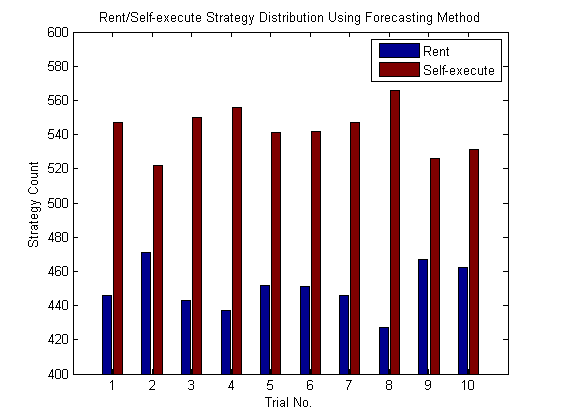
\includegraphics[width=0.9\textwidth]{forecasting1}\\[0.3cm]
\end{center}
An almost equal distribution of strategies of Rent and Self-execute was observed with the game theoretic approach with no strategy overpowering the other. This is because of the randomness in allocating the utility values to the strategies while constructing the matrix. This results in an unbiased evaluation of the matrix which gives an almost equal weightage to both the strategies.
\begin{center}
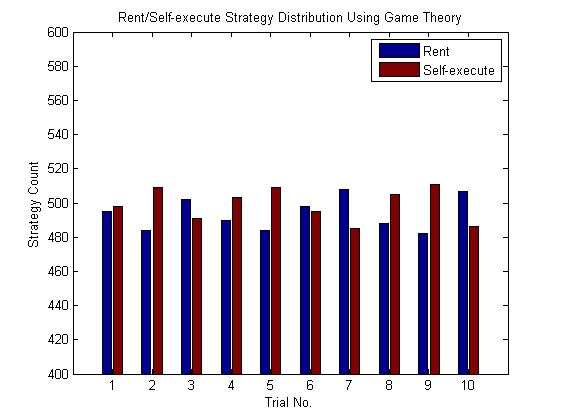
\includegraphics[width=0.9\textwidth]{Gametheory}\\[0.3cm]
\end{center}
The overall strategy also shows an almost equal distribution after resolving the conflicts. In case of conflicts, the final strategy obtained from the standard deviation method considers both forecasting and game theoretic approaches. In this case, the utility values of the jobs in the current batch is compared with the utility values obtained from forecasting and game theory. This method finally selects the strategy that does not deviate much from the expected value obtained from the above two approaches, thus making it easier for the cloud provider to provide the services required to execute the batch without deviating much from the services he already provides.\\[0.3cm]
\begin{center}
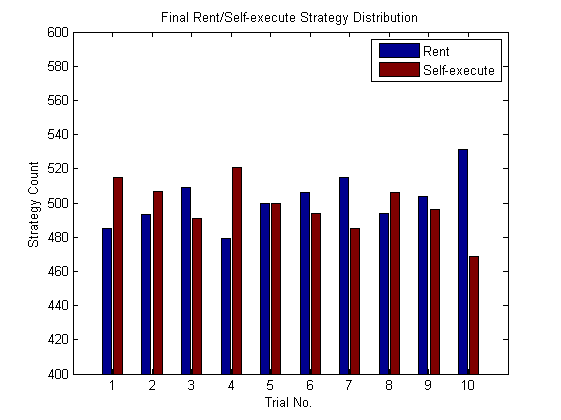
\includegraphics[width=0.9\textwidth]{final}\\[0.3cm]
\end{center}
The results obtained above are with respect to the randomly generated data inputs. In the real environment, certain values like waiting probability depends on factors like network congestion, efficiency of the cloud, datacenter locations, etc. So during run-time, the results obtained may vary with respect to dynamic factors. The utility function can also be further enhanced to include economic factors for the cloud provider to get a clearer picture.

